% $Author: stef $
% $Date: 2008-04-04 17:14:31 +0200 (Fri, 04 Apr 2008) $
% $Revision: 318 $
%=================================================================
\ifx\wholebook\relax\else
% --------------------------------------------
% Lulu:
    \documentclass[a4paper,10pt,twoside]{book}
    \usepackage[
        papersize={6in,9in},
        hmargin={.75in,.75in},
        vmargin={.75in,1in},
        ignoreheadfoot
    ]{geometry}
    \input{../common.tex}
    \pagestyle{headings}
    \setboolean{lulu}{true}
% --------------------------------------------
% A4:
%   \documentclass[a4paper,11pt,twoside]{book}
%   \input{../common.tex}
%   \usepackage{a4wide}
% --------------------------------------------
    \graphicspath{{figures/} {../figures/}}
    \begin{document}
%   \renewcommand{\nnbb}[2]{} % Disable editorial comments
    \sloppy
\fi

\chapter{Des Robots et des Hommes}\label{cha:robots}

\noindent\hrule
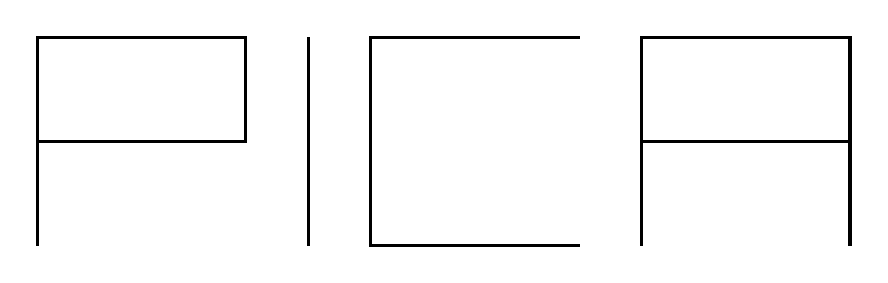
\includegraphics[width=0.9\linewidth]{turtleMPica}
\noindent\hrule\vspace{1.5cm}

Dans ce chapitre je d\'ecris la cr\'eation de robots, les diff\'erents types de mouvements connus 
et ex\'ecutables par les robots. Je vous offre plusieurs exercices simples \`a r\'ealiser. Donc vous 
pouvez mettre en pratique ce que vous avez appris dans les pr\'ec\'edents chapitres. Je vous montrerai 
comment les robots peuvent changer de direction le long de points cardinaux fixes ou \emph{absolus}.


% | caro |
% caro := robot new.
% "letter P"
% caro west; jump: 30 ;jump: 100; north.
% caro go: 100; east; go: 100; south; go: 50.
% caro west; go: 100; south ; jump: 50 ; east.
% caro jump: 130.
% "letter I"
% caro north; go: 100; south; jump: 100; east; jump: 30.
% "letter C" 
% caro jump: 100 ; north;  jump: 100 ; west ; go: 100; 
% south; go: 100; east; go: 100; jump: 30.
% "letter A"
% caro north.
% caro go: 100.
% caro east.
% caro go: 100.
% caro south.
% caro go: 100.
% caro north.
% caro go: 50.
% caro west.
% caro go: 100.



\newpage
\section{Cr\'eation de Robots}

Dans les pr\'ec\'edents chapitres tu as cr\'e\'e \emph{un} robot, et non \emph{le} robot. Les robots ne sont pas uniques et vous 
pouvez en cr\'eer autant que vous voulez. Le Script~\ref{scr:tworobots}cr\'ee 2 robots : pica et daly.

\begin{script}[tworobots]{Deux robots sont n\'es.}
| pica daly | 
pica := Bot new. 
daly := Bot new. 
pica color: Color yellow. 
daly jump: 100. 
\end{script}

La seconde ligne cr\'ee un robot nomm\'e pica comme dans le Script ~\ref{scr:helloworld}. La troisi\`eme ligne cr\'ee un nouveau robot que nous mentionnons en utilisant la variable daly. (Comme le nom de pica est en hommage \`a Pablo Picasso, celui de daly honore Salvador Dali). Les deux robots sont cr\'e\'es aux m\^eme endroit sur l'\'ecran. Dans le 4\`eme ligne, pica est cit\'e pour changer sa couleur en jaune afin de distinguer les deux robots.

Smalltalk est un langage de programmation orient\'e objet, comme je l'avais mentionn\'e. Cela ne 
signifie pas seulement que nous pouvons cr\'e\'er des objets et interagir avec eux, mais que les 
objets peuvent cr\'eer d'autres objets et communiquer avec eux.  De plus, dans  Smalltalk, il y 
a des objets sp\'eciaux, appel\'e classes, qui sont utilis\'ees pour cr\'eer des objets. L'envoie du message\ct{new} 
\`a une classe cr\'ee un objet d\'ecrit par cette classe. L'envoi du message \ct{new} \`a une classe \ct{Bot} cr\'ee un robot. 

Pour comprendre ce que sont des classes, imaginez une classe comme une sorte d'usine. Une usine cr\'eant un moule 
\`a boites  doit produire un grand nombre de boites g\'en\'eriques, tous de la m\^eme taille, m\^eme couleur et m\^eme forme. 
Apr\`es avoir \'et\'e fabriqu\'ees, plusieurs boites seront peut-\^etre remplies de biscuits, tandis que d'autres seront 
peut-\^etre \'ecras\'ees. Quand une boite est \'ecras\'ee, les autres boites ne sont pas touch\'ees. Ce sera la m\^eme chose pour 
les objets cr\'ees \`a l'int\'erieur de Squeak. Dans notre cas, daly ne change pas de couleur, mais pica le fait, alors que 
pica ne bouge pas contrairement \`a daly. Vous pouvez consid\'erer une classe comme une usine capable de produire des 
r\'eserves illimit\'ees d'objets du m\^eme type. Une fois produit, chaque objets existe ind\'ependamment des autres et peut \^etre 
modifi\'e comme on le souhaite.

Dans Smalltalk, les classes sont toujours nomm\'es avec la premi\`ere lettre en majuscule. C'est pourquoi le nom 
de la classe de robot est \ct{Bot} avec un ``B'' majuscule. Notons que dans la commande Color yellow, le mot 
\ct{Color} est \'ecrit avec un ``C'' majuscule. C'est d\^u au fait que \ct{Color}est une classe, et que sa fabrique 
est d'objet couleur. En sp\'ecifiant le nom couleur, vous obtenez un objet de la couleur que vous voulez. 
(L'expression \ct{Color yellow}est actuellement une forme courte pour cr\'eer un objet de couleur jaune. 
Premi\`erement, un objet couleur est cr\'e\'e en envoyant le message\ct{new} \`a la classe \ct{Color},et ensuite 
plusieurs messages suppl\'ementaires d\'efinissent la couleur pour \^etre jaune.) 


\important{Une classe est une usine qui fabrique des objets? En envoyant le message \ct{new} \`a une classe cr\'ee un objet de cette classe. Les noms des classes commencent toujours pas une lettre majuscule. Ici\ct{Bot} est le nom de la fabrique pour cr\'eer de nouveaux robots, et \ct{Color} est la fabrique de couleurs.

 Ainsi la commande \ct{Bot new color: Color blue} envoie un message \`a la classe \ct{Bot} pour cr\'eer un nouveau robot  et envoie ensuite un message au nouveau robot pour sa propre couleur avec la couleur bleue.}


\section{Dessiner des Traits}

Demander \`a un robot de dessiner une ligne est assez simple, comme vous l'avez vu dans le pr\'ec\'edent chapitre. Le message \ct{go: 100} dit au robot de se d\'eplacer de 100 pixels, et le robot laisse une trace pendant son mouvement. Cependant, lorsque vous dessinez, m\^eme si vous \^etes un expert chinois ou japonais en calligraphie, 
vous avez besoin de soulever le crayon de temps en temps. Pour cette intention, un robot sait comment sauter ; 
c'est pourquoi un robot sait se d\'eplacer sans laisser de trace. Un robot comprend le message \ct{jump:}, ainsi que \ct{go:}; qui est une distance donn\'ee en pixel. Le Script~\ref{scr:twolines} dessine deux segments. Pour garder l'image impeccable, j'ai mis les robots en dehors de l'illustration 
en utilisant le message \ct{beInvisible}. 


\begin{script}[twolines]{Pica est cr\'e\'e et ensuite dessine deux lignes.}
!\framebox{
\includegraphics{turtleMTwoLines}}!

| pica | 
pica := Bot new. 
pica go: 30. 
pica jump: 30. 
pica go: 30. 
\end{script}


\begin{experiment}[xp1]{Cr\'eation et Mouvement d'un Robot}
Exercons nous en changeant les valeurs du script pr\'ec\'edent. 
\end{experiment}

\begin{experiment}[sos]{SOS}
Ecrire un script qui dessine le message "SOS" dans le code Morse. (En Morse, un "S" est repr\'esent\'e par trois lignes courtes, et un "O" par trois longues lignes, comme le montre la figure ci-dessous.
 
!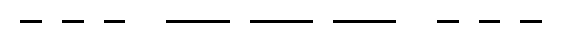
\includegraphics{turtleMSosLines}!
\end{experiment}


\section{Changement de Directions}

Un robot peut lui m\^eme s'orienter le long de huit directions principales d'une boussole, comme le montre la 
Figure~\ref{fig:roseDesVents}. Les directions sont les m\^eme que sur une carte standard : \ct{east} est \`a droite, \ct{west} \`a gauche, \ct{north} au dessus, et \ct{south} en dessous. Ces directions sont absolues, ce qui signifie que sans tenir compte de la direction dans laquelle le robot est en train de pointer, si vous l'appelez au point east, le robot pointera \`a droite de l'\'ecran, et non pas \`a la droite du robot. Pour pointer un robot dans une direction absolue donn\'ee, envoyez juste un message avec le nom de la direction. Ainsi, pour dire \`a pica de s'orienter au sud, vous devez simplement taper \`a la machine 
\ct{pica south}. 

\begin{figure}
\center{\includegraphics[width=10cm]{roseDesVents}}
\caption{Les directions absolues par d\'efaut d'une boussole dans lesquelles un robot peut pointer. 
\label{fig:roseDesVents}}
\end{figure}

Les robots comprennent les messages de direction d'une boussole suivante : \ct{east}, \ct{north}, \ct{northEast}, 
\ct{northWest}, \ct{south}, \ct{southEast}, \ct{southWest}, et \ct{west}. Dans le chapitre suivant, je vous montrerai comment faire tourner un robot avec sa position actuelle et un angle arbitraire. 
Le Script~\ref{scr:gaggle}illustre les quatre directions cardinaux avec quatre robots diff\'erents : 
ici Picasso et Dali ont \'et\'e rejoint par Paul Klee et Alfred Sisley. A l'exception de pica, qui reste 
dans la direction par d\'efaut east dans laquelle il a \'et\'e cr\'e\'e, chaque robot est orient\'e dans une direction 
diff\'erentes avant de lui dire de bouger.


\begin{script}[gaggle]{Un troupeau de robots se prom\`ene.}
| pica daly klee sisl | 
pica := Bot new. 
pica color: Color green. 
pica go: 100. 
daly := Bot new. 
daly north. 
daly color: Color yellow. 
daly go: 100. 
klee := Bot new. 
klee west. 
klee color: Color red. 
klee go: 100. 
sisl := Bot new. 
sisl south. 
sisl go: 100. 
\end{script}

Vous pouvez utiliser ces m\'ethodes d'orientation pour faire des dessins plus complexes. 

\begin{exonofigtitle}{Un Carr\'e}\label{xp:square}
Comme premier exercice, dessinez un carr\'e avec des cot\'es de longueur de 50 pixels. Ensuite dessinez un autre carr\'e de longueur de cot\'e de 250 pixels. 
\end{exonofigtitle}


\begin{exofigwithsize}[0.5]{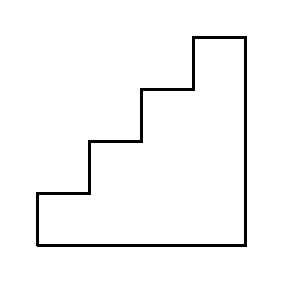
\includegraphics[width=3cm]{turtleMSmallStairs}}{Un Escalier}\label{xp:letterA}
YVous n'\^etes pas limit\'e pour vos dessins avec les robots \`a des carr\'es. Vous pouvez cr\'eer un large \'eventail de figures g\'eom\'etriques. 
Par exemple, nous pouvons voir ici un dessin d'un petit escalier. Ecrivez un script pour reproduire ce dessin.
\end{exofigwithsize}


\begin{exofigwithsize}[0.5]{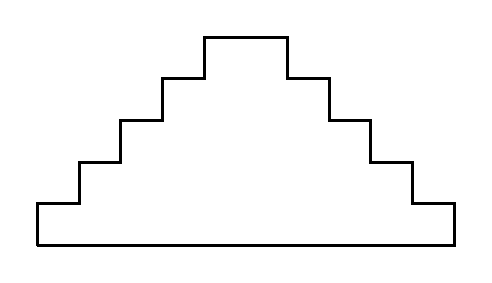
\includegraphics[width=5cm]{turtleMSaqqarah}}{Les Marches de la Pyramide de Saqqara}\label{xp:saqq}
Maintenant vous \^etes pr\`es \`a d\'evelopper votre domaine architectural et dessiner une vue de cot\'e sch\'ematique des marches 
de la pyramide de Saqqara, construite au alentour de 2900 B.C.E. par l'architecte Imhotep. Ecrivez un script pour 
dessiner une vue de cot\'e de cette pyramide, comme le montre la figure. La pyramide a quatre gradins et le sommet 
est deux fois plus large que chaque gradin.
\end{exofigwithsize}

\begin{exofigwithsize}[0.5]{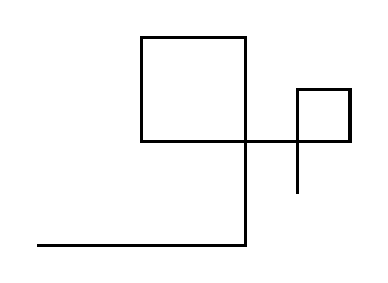
\includegraphics[width=5cm]{turtleMArtNouveau}}{Art abstrait}\label{xp:art}
Ecrivez un script pour dessines l'image montr\'e dans la figure suivante. 
\end{exofigwithsize}


\section{L'ABC du Dessin}

Bien que vous n'ayez pas encore \'enorm\'ement de control sur la direction des traits d'un robot, vous pouvez commencer 
\`a programmer pica pour \'ecrire des lettres. Le script~\ref{scr:letterA} dessine la lettre primitive "A." 


% \begin{script}[a]{La lettre A est d\'essin\'ee.}
% 	!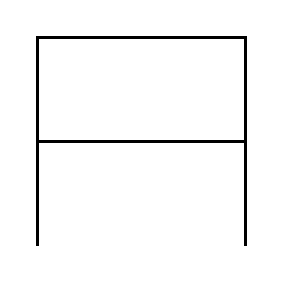
\includegraphics{turtleMLetterA}!
% 	| pica | 
% 	pica := Bot new. 
% 	pica north. 
% 	pica go: 100. 
% 	pica east. 
% 	pica go: 100. 
% 	pica south. 
% 	pica go: 100. 
% 	pica north. 
% 	pica go: 50. 
% 	pica west. 
% 	pica go: 100 
% \end{script}

\begin{scriptfigwithsize}[0.4]{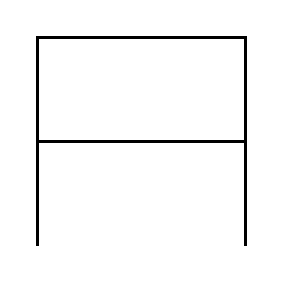
\includegraphics[width=5cm]{turtleMLetterA}}{La Lettre A}\label{scr:letterA}
	| pica | 
	pica := Bot new. 
	pica north. 
	pica go: 100. 
	pica east. 
	pica go: 100. 
	pica south. 
	pica go: 100. 
	pica north. 
	pica go: 50. 
	pica west. 
	pica go: 100
\end{scriptfigwithsize}




Dessiner une lettre "C" n'est pas plus difficile. Vous pouvez m\^eme \'ecrire un script pour \'epeler "PICA".


\begin{exonofigtitle}{Pica}\label{pica}
Dessinez le nom "PICA" comme le montre le d\'ebut de ce chapitre. Pour s\'eparer les lettres individuelles, vous devez utiliser la commande  \ct{jump:}.
\end{exonofigtitle}	
	
	
\note{On peut d\'ebattre sur le fait que le Script 3-4 peut \^etre am\'elior\'e. Par exemple, 
la derni\`ere moiti\'e de la ligne vertical du cote droit de "A" est dessin\'e deux fois, 
lorsque le robot revient sur ce segment -- une fois vers le sud, une fois vers le 
nord -- pour retourner \`a la position  afin de dessiner la barre horizontal. Se d\'ecider pour 
la meilleure approche afin de r\'esoudre un probl\`eme de programmation peut \^etre difficile. Il y a 
plusieurs issues \`a consid\'erer, tel que la vitesse, la complexit\'e, la rentabilit\'e du code, et ces 
questions qui auront diff\'erentes r\'eponses d\'ependant du langage de programmation et des m\'ethodes utilis\'ees. 
Toutefois, une approche que vous devrez consid\'erer est de commencer par choisir la plus simple des solutions. 
Ensuite si vous n'\^etes pas satisfait du \`a la lenteur du programme ou au manque d'options particuli\`eres que 
vous souhaitiez avoir, vous pouvez toujours modifier sa vitesse ou ajouter d'autres am\'eliorations.}	
	
	
\section{Commander la Visibilit\'e du Robot}

Vous pouvez contrôler le fait qu'un robot soit apparent ou pas en utilisant les messages \ct{beInvisible} et 
\ct{beVisible}. Le message \ct{beInvisible} permet de cacher le r\'ecepteur du message. Un robot cach\'e agit exactement 
de la m\^eme mani\`ere qu'un robot apparent ; c'est juste qu'il ne montre pas où il est. Attention a ne pas utiliser la m\'ethode 
\ct{hide}, qui est d\'efini par Squeak pour lui m\^eme et peut endommager l'environnement si on l'utilise de façon incorrect. 
Le message\ct{beVisible} rend visible le robot recevant ce message. Un nouveau robot cr\'e\'e est visible par d\'efaut. 

\section{R\'esum\'e}

Le tableau suivant r\'esume les expressions et messages contenues dans ce chapitre. 

\noindent
\setlength{\extrarowheight}{1mm}
{\small \begin{tabular}{p{30mm}p{50mm}p{30mm}}
\hline
\textbf{Expressions / Messages}&\textbf{Description}&\textbf{Exemple}\\\hline
\textsf{Bot new}&Cr\'ee un robot. &\textsf{pica := Bot new}\\
\textsf{$|$ x y $|$}
&
D\'eclare les variables pour \^etre 
utilis\'ees dans le script \emph{script}
&
\textsf{$|$ pica $|$}
\\
\textsf{jump: {\itshape anInteger}}
&

Dit au robot de se d\'eplacer 
du nombre donn\'e de pixels 
sans laisser une trace. 

&
\textsf{pica jump: 10}
\\
\textsf{go: {\itshape unEnter}}
&

Dit au robot de se d\'eplacer 
du nombre donn\'e de pixels 
tout en laissant une trace. 

&
\textsf{pica go: 10}
\\
\textsf{beInvisible}
&
Dit au robot d'\^etre invisible.
&
\textsf{pica beInvisible}
\\
\textsf{beVisible}
&
Dit au robot d'\^etre visible.
&
\textsf{pica beVisible}
\\
\textsf{east, northEast, north, northWest, west, southWest, south, southEast.}
&

Dit au robot de pointer dans 
la direction donn\'ee. 

&
\textsf{pica north}
\\
\textsf{Color {\itshape colorName}}
&
Cr\'ee une couleur \textit{colorName}
&
\textsf{Color blue}
\\
\textsf{color: {\itshape aColor}}
&
Demande au robot de changer sa couleur.
&
\textsf{pica color: Color red}
\\
\hline
\end{tabular}}


	
\ifx\wholebook\relax\else
    \end{document}
\fi

%%% Local Variables:
%%% coding: utf-8
%%% mode: latex
%%% TeX-master: t
%%% TeX-PDF-mode: t
%%% ispell-local-dictionary: "english"
%%% End:
